%% liftarm.tex
%% Copyright 2022 Matthias Floré
%
% This work may be distributed and/or modified under the
% conditions of the LaTeX Project Public License, either version 1.3
% of this license or (at your option) any later version.
% The latest version of this license is in
%   http://www.latex-project.org/lppl.txt
% and version 1.3 or later is part of all distributions of LaTeX
% version 2005/12/01 or later.
%
% This work has the LPPL maintenance status `maintained'.
% 
% The Current Maintainer of this work is Matthias Floré.
%
% This work consists of the files liftarm.pdf, liftarm.sty,
% liftarm.tex and README.md.
\documentclass[a4paper,english,dvipsnames]{ltxdoc}
\usepackage[english]{babel}
\usepackage{graphicx}
\usepackage[a4paper,left=2.25cm,right=2.25cm,top=2.5cm,bottom=2.5cm,nohead]{geometry}
\usepackage{parskip}
\usepackage[T1]{fontenc}
\usepackage[utf8]{inputenc}
\usepackage{mathtools}
\usepackage{amssymb}
\allowdisplaybreaks
\usepackage{multicol}
\usepackage{animate}
\usepackage{liftarm}
\input{pgfmanual-en-macros.tex}
\usepackage[page]{totalcount}
\usepackage{fancyhdr}
\pagestyle{fancy}
\renewcommand{\headrulewidth}{0pt}
\cfoot{\iftotalpages\begin{tikzpicture}\liftarm[mark holes=\thepage-1]{0,0}{\totalpages-2}{0}\end{tikzpicture}\fi}%\liftarm{0,0}{\thepage}{0}
\fancyhead{}
\usepackage{imakeidx}
\makeindex[program=makeindex,columns=2,intoc=true]
\indexsetup{othercode={\thispagestyle{fancy}}}
\usepackage[linktoc=all,pdfstartview=FitH,colorlinks=true,linkcolor=Mahogany,citecolor=ForestGreen,urlcolor=MidnightBlue,bookmarksnumbered=true]{hyperref}
\hypersetup{pdftitle={The liftarm package},pdfauthor={Matthias Flor\'e},pdfsubject={Manual},pdfkeywords={liftarm}}
\setcounter{tocdepth}{2}
\setcounter{secnumdepth}{2}
\DeclareMathOperator{\atan}{atan}
\title{The \texttt{liftarm} package\\[12pt]\large Draw liftarms with \tikzname}
\author{Matthias Flor\'e}
\date{Version 2.0 (2022/04/07)}%\\[12pt]
\begin{document}
\maketitle
\thispagestyle{fancy}
\begin{abstract}
\noindent This package is based on the package |tikz| (see \cite{TtTaPGFp}) and can be used to draw liftarms with \tikzname. It provides several options for the appearance of the liftarms, a command which connects two liftarms, an environment to describe a construction and a method to animate a construction with one or more traces.% This is the manual for version .
\end{abstract}
\tableofcontents
\section{Usage}
The package |liftarm| can be used by putting the following in the preamble.
\begin{codeexample}[code only]
\usepackage{liftarm}
\end{codeexample}
The package |liftarm| loads the packages |etoolbox|, |xcolor| with the option |dvipsnames|, |tikz| and the \tikzname{} library |calc|. Since |xcolor| is loaded with the option |dvipsnames|, packages such as |pgfplots| and |tcolorbox| must be loaded \emph{after} |liftarm|.
\section{Drawing liftarms}
\begin{command}{\liftarm\opt{\oarg{options}}\marg{point}\marg{length}\marg{angle}}
This command can be placed inside a |tikzpicture| environment. It draws a liftarm of \meta{length} starting at \meta{point}. The angle between the liftarm and the $x$-axis can be specified by \meta{angle} in degrees. The distance between the holes is $1$.
\begin{codeexample}[width=10cm]
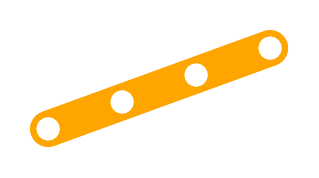
\begin{tikzpicture}
\liftarm{1,2}{3}{20}
\end{tikzpicture}
\end{codeexample}
Note that the number of holes is $\meta{length}+1$. The \meta{options} can be given with the following keys.
\begin{key}{/liftarm/axle holes=\marg{values}}
This key defines the holes in the liftarm where axle holes will be drawn.
\begin{codeexample}[width=10cm]

\begin{tikzpicture}
\liftarm[axle holes={0,4}]{0,1}{4}{0}
\end{tikzpicture}
\end{codeexample}
\end{key}
\begin{key}{/liftarm/brick=\opt{\meta{boolean}} (default true, initially false)}
If true, a brick will be drawn instead of a liftarm.
\begin{codeexample}[width=10cm]

\begin{tikzpicture}
\liftarm[brick]{0,1}{2}{0}
\end{tikzpicture}
\end{codeexample}
\end{key}
\begin{key}{/liftarm/color=\marg{name}}
This key defines the color of the liftarm. The color can also be specified without key.
\begin{codeexample}[width=10cm]
\begin{tikzpicture}
\liftarm[color=Green]{0,1}{4}{0}
\liftarm[Blue]{0,2}{3}{0}
\end{tikzpicture}
\end{codeexample}
\end{key}
\begin{key}{/liftarm/color 0=\marg{name} (initially Gray)}
\end{key}
\begin{key}{/liftarm/color 1=\marg{name} (initially darkgray)}
\end{key}
\begin{key}{/liftarm/color 2=\marg{name} (initially Yellow)}
\end{key}
\begin{key}{/liftarm/color 3=\marg{name} (initially Orange)}
\end{key}
\begin{key}{/liftarm/color 4=\marg{name} (initially Red)}
\end{key}
\begin{key}{/liftarm/color 5=\marg{name} (initially Green)}
\end{key}
\begin{key}{/liftarm/color 6=\marg{name} (initially Blue)}
\end{key}
\begin{key}{/liftarm/color 7=\marg{name} (initially Brown)}
These keys define the colors of the liftarms which have as their length the number following |color|.
\end{key}
\begin{key}{/liftarm/color modulo=\marg{number} (initially 8)}
The default colors of the liftarms are determined by computing the length of the liftarm modulo the value of this key and selecting the color from the previous keys.
\begin{codeexample}[width=10cm]
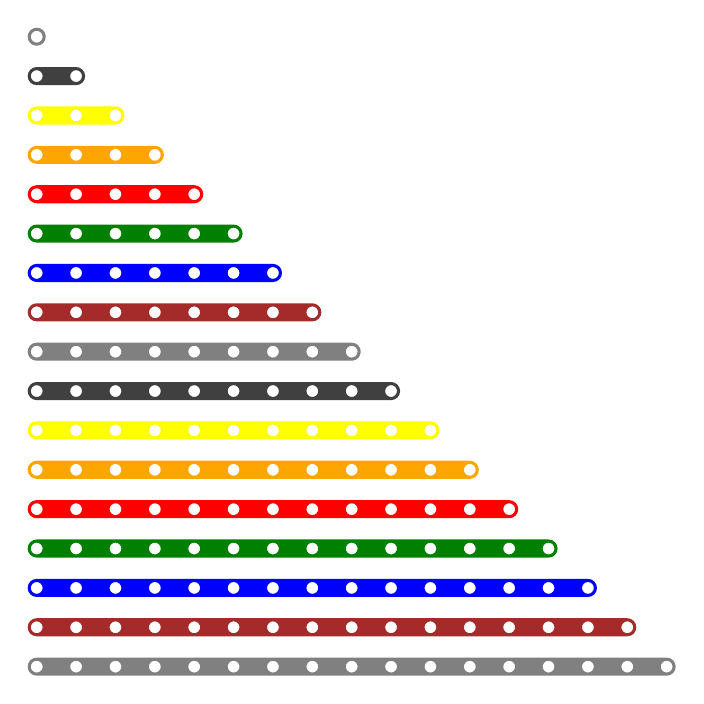
\begin{tikzpicture}[scale=0.5]
\foreach\n in {0,...,16}{
    \liftarm{0,-\n}{\n}{0}
}
\end{tikzpicture}
\end{codeexample}
\begin{codeexample}[width=10cm]
\begin{tikzpicture}[scale=0.5]
\pgfkeys{
    /liftarm,
    color 0=Yellow,
    color 1=Red,
    color 2=Green,
    color 3=Blue,
    color modulo=4
}
\foreach\n in {0,...,8}{
    \liftarm{0,-\n}{\n}{0}
}
\end{tikzpicture}
\end{codeexample}
\end{key}
\begin{key}{/liftarm/contour=\opt{\meta{boolean}} (default true, initially false)}
If true, a contour will be drawn around the liftarm.
\begin{codeexample}[width=10cm]
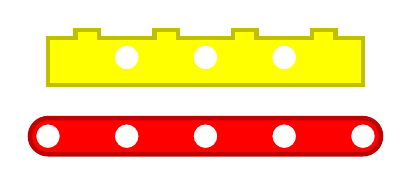
\begin{tikzpicture}
\liftarm[contour]{0,1}{4}{0}
\liftarm[brick,contour]{1,2}{2}{0}
\end{tikzpicture}
\end{codeexample}
\end{key}
\begin{key}{/liftarm/coordinate=\marg{number 1/name 1}\dots}
This key defines coordinates with name \meta{name i} at hole \meta{number i} of the liftarm.
\begin{codeexample}[width=10cm]
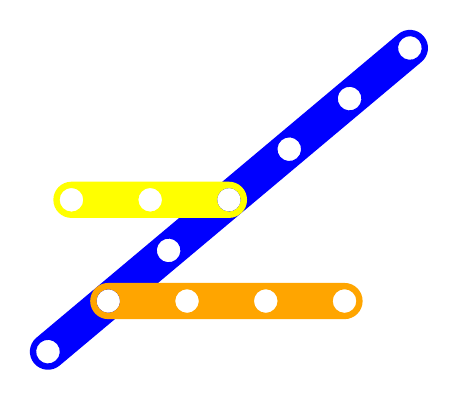
\begin{tikzpicture}
\liftarm[
    coordinate={1/A,3/B}
]{0,1}{6}{40}
\liftarm{A}{3}{0}
\liftarm{B}{2}{180}
\end{tikzpicture}
\end{codeexample}
\end{key}
\begin{key}{/liftarm/hole radius=\marg{value} (initially 0.3)}
The \meta{value} of this key, multiplied with the \meta{value} of the key |scalefactor| defines the radius of the holes.
\begin{codeexample}[width=10cm]

\begin{tikzpicture}
\liftarm[hole radius=0.1]{0,0}{5}{0}
\end{tikzpicture}
\end{codeexample}
\end{key}
\begin{key}{/liftarm/liftarm thickness=\marg{value} (initially 0.92)}
The \meta{value} of this key, multiplied with the \meta{value} of the key |scalefactor| defines the thickness of the liftarm.
\begin{codeexample}[width=10cm]

\begin{tikzpicture}
\liftarm[
    hole radius=0.1,
    liftarm thickness=0.3
]{0,0}{5}{0}
\end{tikzpicture}
\end{codeexample}
\end{key}
\begin{key}{/liftarm/mark color=\marg{name} (initially Black)}
\end{key}
\begin{key}{/liftarm/mark holes=\marg{values}}
The key |mark holes| defines the holes in the liftarm which will be marked. The key |mark color| defines the color of these marks.
\begin{codeexample}[width=10cm]
\begin{tikzpicture}
\liftarm[
    mark holes={0,1,3}
]{0,0}{5}{0}
\liftarm[
    mark holes={1,2,4},
    mark color=Blue
]{0,1}{4}{0}
\end{tikzpicture}
\end{codeexample}
\end{key}
\begin{key}{/liftarm/origin=\marg{number} (initially 0)}
This key defines the number of the hole which will be placed at the coordinate given as argument to the liftarm.
\begin{codeexample}[width=10cm]
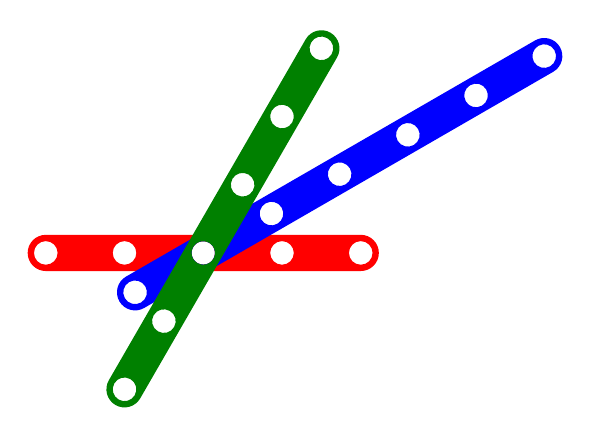
\begin{tikzpicture}
\liftarm{-2,0}{4}{0}
\liftarm[origin=1]{0,0}{6}{30}
\liftarm[origin=2]{0,0}{5}{60}
\end{tikzpicture}
\end{codeexample}
\end{key}
\begin{key}{/liftarm/scalefactor=\marg{value} (initially 0.5)}
The \meta{value} of this key defines the factor which scales the thickness of the liftarm and the radius of the holes.
\begin{codeexample}[width=10cm]
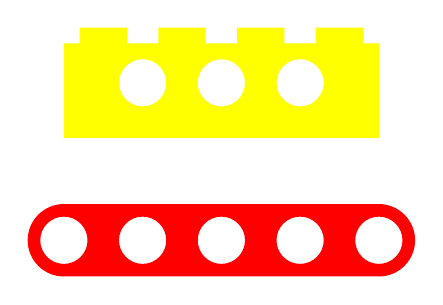
\begin{tikzpicture}
\liftarm[scalefactor=1]{0,0}{4}{0}
\liftarm[brick,scalefactor=1]{1,2}{2}{0}
\end{tikzpicture}
\end{codeexample}
\end{key}
\begin{key}{/liftarm/screw color=\marg{name} (initially Black)}
\end{key}
\begin{key}{/liftarm/screw holes=\marg{values}}
\end{key}
\begin{key}{/liftarm/screw holes angle=\marg{angle} (initially 45)}
The key |screw holes| defines the holes in the liftarm where a screw will be drawn. The key |screw color| defines the color of these screws. The key |screw holes angle| defines the angle in degrees around which the screws are drawn.
\begin{codeexample}[width=10cm]
\begin{tikzpicture}
\liftarm[
    screw holes={0,1,3}
]{0,0}{5}{0}
\liftarm[
    screw holes={1,2,4},
    screw color=Blue,
    screw holes angle=0
]{0,1}{4}{0}
\end{tikzpicture}
\end{codeexample}
\end{key}
\end{command}
\section{Connecting liftarms}
\begin{command}{\liftarmconnect\opt{\oarg{options}}\marg{point1}\marg{length1}\marg{point2}\marg{length2}}
This command can be placed inside a |tikzpicture| environment. It draws a liftarm of \meta{length1} starting at \meta{point1} and a liftarm of \meta{length2} starting at \meta{point2} in such a way that their last holes have the same coordinate in case that such a point exists. If such a point does not exist then nothing is drawn. In case that there exist 2 such points then this point is chosen counterclockwise. In that case, the other configuration of the 2 liftarms can be obtained by simply swapping \marg{point1}\marg{length1} and \marg{point2}\marg{length2}. The keys for the command |\liftarm| can be given to the \meta{options}. In this case these keys will be passed to both liftarms.
\begin{codeexample}[width=9cm]
\begin{tikzpicture}
\coordinate (A) at (0,0);
\coordinate (B) at (4,2);
\coordinate (C) at (1,-3);
\coordinate (D) at (5,-1);
\liftarmconnect[Yellow]{A}{2}{B}{3}
\liftarmconnect[Red]{B}{3}{A}{2}
\liftarmconnect[Green]{C}{3}{D}{2}
\liftarmconnect[Blue]{D}{2}{C}{3}
\foreach\coord in {A,B,C,D}{
    \node at (\coord) {{\small $\coord$}};
}
\end{tikzpicture}
\end{codeexample}
Additionally, the \meta{options} can be given with the following keys.
\begin{key}{/liftarm/connect coordinate=\marg{name}}
This key defines a coordinate with name \meta{name} at the connection point of both liftarms.
\begin{codeexample}[width=10cm]
\begin{tikzpicture}
\liftarm{-3,0}{5}{0}
\liftarmconnect[
    connect coordinate=A
]{2,0}{2}{-2,0}{3}
\liftarm{A}{4}{180}
\end{tikzpicture}
\end{codeexample}
\end{key}
\begin{key}{/liftarm/connect reverse=\opt{\meta{boolean}} (default true, initially false)}
If true, the first liftarm of |\liftarmconnect| will be drawn second and the second liftarm will be drawn first. This option can be used to change the appearance at the connection point of both liftarms.
\begin{codeexample}[width=10cm]
\begin{tikzpicture}
\liftarmconnect{2,0}{1}{0,0}{2}
\liftarmconnect[
    connect reverse
]{5,0}{1}{3,0}{2}
\end{tikzpicture}
\end{codeexample}
\end{key}
\begin{stylekey}{/liftarm/liftarm 1=\marg{options} (initially \normalfont empty)}
\end{stylekey}
\begin{stylekey}{/liftarm/liftarm 2=\marg{options} (initially \normalfont empty)}
These keys accept a list of keys which will be applied to the first respectively second liftarm. These lists of keys accept the same options as the command |\liftarm|. Additionally, the key |connect| below can be given.
\begin{key}{/liftarm/connect=\marg{number}}
This key defines the number of the hole which will be connected to the matching liftarm. If this key is not given then the last hole of the liftarm is taken as the connecting point.
\begin{codeexample}[width=10cm]
\begin{tikzpicture}
\liftarm{0,-7}{10}{90}
\liftarmconnect[
    connect coordinate=A,
    liftarm 1={
        origin=1,
        connect=5
    },
    liftarm 2={
        origin=2,
        connect=6
    }
]{0,2}{6}{0,0}{7}
\liftarmconnect[
    liftarm 1={
        origin=2,
        connect=8
    },
    liftarm 2={
        origin=1,
        connect=5,
        coordinate=4/B
    }
]{A}{9}{0,-6}{6}
\liftarm[origin=1]{B}{4}{70}
\end{tikzpicture}
\end{codeexample}
\end{key}
\end{stylekey}
\end{command}
\section{Describing a construction}
If a construction involves many liftarms then it is convenient to describe this construction in separate steps and |tikzpicture|s. Then the content of previous |tikzpicture|s would need to be copied in each new |tikzpicture|. This process can be automated by using the |liftarmconstruction| environment and the command |\liftarmconstruct| below.
\begin{environment}{{liftarmconstruction}\opt{\oarg{options}}}
This environment is in fact an |enumerate| environment with the addition that it resets the content of the |tikzpicture| which is displayed by the command |\liftarmconstruct| below. Thus in particular, |\item| can be used inside the |liftarmconstruction| environment. The \meta{options} will be passed to each |tikzpicture| drawn by the command |\liftarmconstruct| inside this environment. The following command can be used inside this environment.
\begin{command}{\liftarmconstruct\opt{\oarg{options}}\marg{text}\marg{commands}}
This command starts an |\item| and shows \meta{text}. Then it displays a |tikzpicture| containing \meta{commands} and also the \meta{commands} of previous |\liftarmconstruct| commands inside the same |liftarmconstruction| environment. The \meta{options} will be added to this |tikzpicture| but \emph{only} in the current step.

As an example, we describe below the construction of a regular pentagon from \cite{Tmm1}.
\begin{codeexample}[width=10cm]
\begin{minipage}{0.5\linewidth}%only for
%usage in this manual%\linewidth-6pt
%\begin{multicols}{2}%only for
%usage in this manual
\begin{liftarmconstruction}[scale=0.75]
\liftarmconstruct[
    {\node[left,align=left]
        at (-0.5,-1.3)
        {Rectangular triangle.\\
        This text is only\\
        visible in this step.};}
]{
    We start with 3 liftarms to form
    a rectangular triangle.
}{
\liftarm{-3,0}{4}{0}
\liftarmconnect[
    liftarm 1={
        origin=2,
        mark holes={2,6}
    },
    liftarm 2={
        mark holes=0
    }
]{0,0}{6}{-3,0}{5}}
\item An |\item| can be added since this
    is an |enumerate| environment.
\liftarmconstruct{
    Now we add 2 liftarms of length $3$.
}{\liftarmconnect[
    connect coordinate=A,
    liftarm 1={
        mark holes={0,3}
    },
    liftarm 2={
        mark holes=0
    }
]{0,-2}{3}{0,2}{3}}
\liftarmconstruct{
    In this step we construct the first
    side of the regular pentagon.
}{\liftarmconnect[
    connect coordinate=B,
    liftarm 2={
        mark holes={0,2}
    }
]{A}{2}{1,0}{2}}
\liftarmconstruct{
    Now we finish the construction
    of the regular pentagon.
}{\liftarmconnect[
    liftarm 2={
        mark holes={0,2}
    }
]{B}{2}{-1,0}{2}
\liftarmconnect[
    liftarm 1={
        mark holes=2
    }
]{-1,0}{2}{A}{2}}
\end{liftarmconstruction}
%\end{multicols}
\end{minipage}
\end{codeexample}
\end{command}
\end{environment}
\section{Animations}
\begin{command}{\liftarmanimate\opt{\oarg{options}}\marg{frame rate}\marg{list}\marg{command}}
This command shows an animation using the |animateinline| environment of the package |animate|. The package |animate| is \emph{not} loaded by default and needs to be loaded to use the command |\liftarmanimate|. The \meta{options} are passed to the |animateinline| environment. The \meta{frame rate} of the animation is described in the documentation of the package |animate|. The \meta{command} must be a previously defined command with one mandatory argument. The \meta{list} is passed to a |\foreach| loop. The frames of the animation consist of the \meta{command} evaluated one by one in the result of the |\foreach| loop. The command |\liftarmanimate| creates a timeline which is used in the |animateinline| environment. This timeline is stored in the file |liftarm|\meta{number of the animation in the document}|.tln|. It requires two compiler runs to create and use this timeline correctly.
\begin{key}{/liftarm/trace=\marg{number/number of frames/code}\dots}
This key draws \meta{code} at hole \meta{number} of the liftarm on the frames of the animation determined by \meta{number of frames}.

If \meta{number of frames} is 0 then the \meta{code} is drawn starting at the current frame until the end of the animation. If \meta{number of frames} is an integer greater than or equal to 1 then the \meta{code} is drawn starting at the current frame and remaining during the next frames determined by \meta{number of frames}. If \meta{number of frames} is left empty then the \meta{code} is drawn starting at the beginning of the animation until the end of the animation.

The \meta{code} can be some \tikzname{} code. In this \meta{code}, $(0,0)$ is positioned at hole \meta{number} of the liftarm. If \meta{code} is left empty then the following code is used.
\begin{codeexample}[code only]
\fill[Black] (0,0) circle[radius=0.66*\liftarm@holeradius];
\end{codeexample}
A list of multiple triples \meta{number/number of frames/code} can be given to the key |trace|.
\begin{codeexample}[width=10cm,preamble={\usepackage{animate}}]
\newcommand{\exampleliftarmanimate}[1]{
    \liftarm[
        origin=1,
        mark holes=1,
        trace={
            2/0/,
            3//,
            4/3/{\fill[Blue] (0,0)
                circle[radius=0.15];}
        }
    ]{0,0}{4}{#1}
}
\liftarmanimate[
    autoplay,
    controls,
    loop,
    begin={
        \begin{tikzpicture}
        \useasboundingbox (-4,-4)
            rectangle (4,4);
    },
    end={\end{tikzpicture}}
]
{5}
{0,30,...,330}
{\exampleliftarmanimate}
\end{codeexample}
\end{key}
\end{command}
\section{Additional examples}
The following example shows a regular hexagon.
\begin{codeexample}[width=9cm]
\begin{tikzpicture}
\def\r{3}
\foreach\n in {1,...,6}{
    \liftarmconnect{0,0}{\r}{\n*60:\r}{\r}
}
\end{tikzpicture}
\end{codeexample}
The following example illustrates that $2\atan(\frac{1}{2})=\atan(\frac{4}{3})$.
\begin{codeexample}[width=9cm]
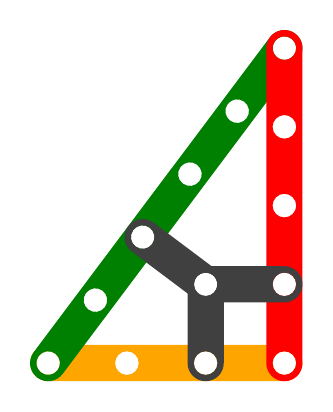
\begin{tikzpicture}
\liftarm{0,0}{3}{0}
\liftarm{0,0}{5}{atan(4/3)}
\liftarm{3,0}{4}{90}
\liftarm{2,0}{1}{90}
\liftarm{2,1}{1}{0}
\liftarm{2,1}{1}{90+atan(4/3)}
\end{tikzpicture}
\end{codeexample}
Below is an example of an angled liftarm.
\begin{codeexample}[width=9cm]
\begin{tikzpicture}
\pgfkeys{
    /liftarm,
    scalefactor=1,
    Blue
}
\liftarm[axle holes=0]{0,0}{3}{0}
\liftarm[axle holes=5]{3,0}{5}{atan(4/3)}
\end{tikzpicture}
\end{codeexample}
The following example illustrates an angle bisection.
\begin{codeexample}[width=9cm]
\begin{tikzpicture}
\def\ang{40}
\def\r{3}
\liftarm[mark holes={0,\r}]{0,0}{2*\r}{0}
\liftarm[mark holes=\r]{0,0}{2*\r}{\ang}
\liftarm[
    mark holes=\r,
    mark color=Red
]{\r,0}{\r}{\ang}
\liftarm{\ang:\r}{\r}{0}
\end{tikzpicture}
\end{codeexample}
The following example illustrates that $7^{2}+4^{2}=8^{2}+1^{2}$.
\begin{codeexample}[width=9cm]
\begin{tikzpicture}[scale=0.75]
\def\a{4}
\def\b{7}
\def\c{1}
\def\d{8}
%\liftarm{0,0}{\b}{0}
%\liftarm{\b,0}{\a}{90}
\liftarmconnect{0,0}{\b}{\b,\a}{\a}
\liftarm{4,0}{3}{90}
%\liftarm{\b,\a}{1}{atan(\a/\b)+atan(\c/\d)+90}
%\liftarm{0,0}{\d}{atan(\a/\b)+atan(\c/\d)}
\liftarmconnect{\b,\a}{\c}{0,0}{\d}
\end{tikzpicture}
\end{codeexample}
Below is an animation of the Peaucellier-Lipkin linkage, see e.g.~\cite{Koagmopermbl}.
\begin{codeexample}[width=9cm,preamble={\usepackage{animate}}]
\newcommand{\PLlinkage}[1]{
\begin{tikzpicture}[scale=0.75]
\def\a{3}
\def\b{4}
\def\c{9}
\pgfmathsetmacro{\x}{
    2*\a+((\c^2-\b^2-(2*\a)^2)/(2*\a))
}
\useasboundingbox (-0.23,-6) rectangle
    ({\x+0.23},6);
\draw (\x,-5)--(\x,5);
\liftarm{0,0}{\a}{0}
\liftarm[coordinate=\a/A]{\a,0}{\a}{#1}
\liftarmconnect[
    connect coordinate=B,
    connect reverse
]{A}{\b}{0,0}{\c}
\liftarmconnect[
    connect coordinate=C
]{0,0}{\c}{A}{\b}
\liftarmconnect{C}{\b}{B}{\b}
\end{tikzpicture}
}
\begin{animateinline}[
    autoplay,
    controls,
    palindrome
]{30}
\multiframe{80}{rAng=-40+1}{
    \PLlinkage{\rAng}
}
\end{animateinline}
\end{codeexample}
Below is an animation of Kempe's trisector, as shown in \cite{Tmm3}.
\begin{codeexample}[preamble={\usepackage{animate}}]
\newcommand{\trisector}[1]{
\begin{tikzpicture}[scale=0.33]
\useasboundingbox (-27.3,-0.5) rectangle (21.2,37);
\liftarm[coordinate=8/A]{0,0}{27}{180}
\liftarm[coordinate=12/B]{0,0}{27}{180-(#1)}
\liftarm[coordinate=18/C]{0,0}{27}{180-2*(#1)}
\liftarm[coordinate=27/D]{0,0}{27}{180-3*(#1)}
\liftarmconnect{C}{27}{D}{18}
\liftarmconnect[liftarm 2={connect=8}]{A}{12}{B}{18}
\end{tikzpicture}
}
\begin{animateinline}[autoplay,controls,palindrome]{5}
\multiframe{20}{rAng=15+1}{
\trisector{\rAng}
}
\end{animateinline}
\end{codeexample}
Below is an animation of Chebyshev's Lambda Mechanism.
\begin{codeexample}[width=10cm,preamble={\usepackage{animate}}]
\newcommand{\CL}[1]{
\liftarm{0,0}{4*\r}{0}
\liftarm[
    mark holes={0,2*\r}
]{0,0}{2*\r}{#1}
\liftarmconnect[
    liftarm 1={mark holes={0,5*\r}},
    liftarm 2={
        connect=5*\r,
        mark holes=10*\r,
        mark color=Red,
        trace={6*\r/0/,10*\r//}
    }
]{4*\r,0}{5*\r}{#1:2*\r}{10*\r}
}
\liftarmanimate[
    autoplay,
    controls,
    loop,
    begin={
        \begin{tikzpicture}[scale=0.8]
        \def\r{1}
        \useasboundingbox
            (-2*\r-0.5,-2*\r-0.5)
            rectangle
            (10*\r-0.5,10*\r+0.5);
    },
    end={\end{tikzpicture}}
]
{20}
{0,5,...,355}
{\CL}
\end{codeexample}
\section{Version history}
\begin{itemize}
\item[] \textbf{Version 1.0 (2022/03/08)} First version.
\item[] \textbf{Version 2.0 (2022/04/07)} Removed some redundant |;| in the code.\footnote{Thanks to Denis Bitouz\'e for pointing this out.} Added the command |\liftarmanimate| and the key |trace|.
\end{itemize}
\begin{thebibliography}{9}
\bibitem{Tmm1}
Gerard 't Hooft,
\emph{Meccano Math I},\\
\url{https://webspace.science.uu.nl/~hooft101/lectures/meccano.pdf},
2006.
\bibitem{Tmm2}
Gerard 't Hooft,
\emph{Meccano Math II},\\
\url{https://webspace.science.uu.nl/~hooft101/lectures/meccano2.pdf},
2008.
\bibitem{Tmm3}
Gerard 't Hooft,
\emph{Meccano Math III},\\
\url{https://webspace.science.uu.nl/~hooft101/lectures/meccano3.pdf},
2014.
\bibitem{Koagmopermbl}
Alfred Bray Kempe,
\emph{On a general method of producing exact rectilinear motion by linkwork},
1875.
\bibitem{TtTaPGFp}
Till Tantau,
\emph{The \tikzname{} and {\upshape\pgfname} Packages},
Manual for version 3.1.9a,
\url{https://ctan.org/pkg/pgf},
2021.
\end{thebibliography}
\printindex
\end{document}